\documentclass{article}
\usepackage{amsmath}
\usepackage{graphicx}
\usepackage{graphics}
\usepackage{amssymb}
\usepackage{booktabs}
\usepackage{listings}
\usepackage{color}
\usepackage{caption}
\usepackage{subcaption}
\usepackage[margin=0.8in]{geometry}

\definecolor{dkgreen}{rgb}{0,0.6,0}
\definecolor{gray}{rgb}{0.5,0.5,0.5}
\definecolor{mauve}{rgb}{0.58,0,0.82}

\begin{document}
\title{Homework 3 \\CS 5220}
\author{Lara Backer, Greg Granito, Sam Tung}

\maketitle

%%%%%%%%%%%%%%%%%%%%%%%%%%%%%%%%%%%%%%%%%%%%%%%%%%%%%%%%%%%%%%%%%%%%%%%
\section{Introduction}

\section{Base OpenMP Code}

\subsection{Profiling}
A look into performance of the code was conducted by using Intel's VTUNE on Totient. Due to some technical issues with the cluster, we could not run the "advanced-hotspots" for profiling. 
	\begin{figure}[h!]
		\begin{center}
			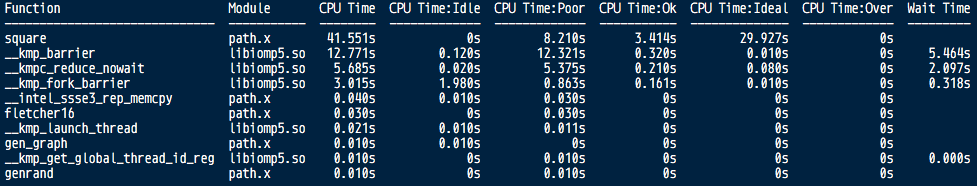
\includegraphics[width=0.7\columnwidth]{amplxe}
			\caption{Most time consuming functions in the base code.}
			\label{amplxe}
		\end{center}
	\end{figure}
	
From looking at VTUNE, it appears that the most time spent in the program was done on the square function. This is not surprising, as there are plenty of nested for loops in the code, which undoubtedly takes a while to run through.

\subsection{Scaling}

\section{OpenMPI}

\subsection{Profiling}
After attempting to implement OpenMPI, we once again look into performance of the code through profiling. 
	\begin{figure}[h!]
		\begin{center}
			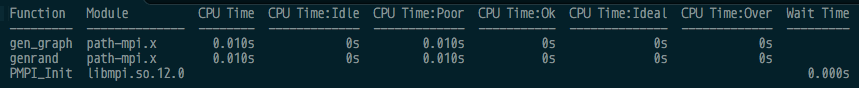
\includegraphics[width=0.7\columnwidth]{amplxe_mpi}
			\caption{Most time consuming functions in the OpenMPI implementation.}
			\label{amplxe_mpi}
		\end{center}
	\end{figure}

\subsection{Scaling}

\section{Processor Offloading}

\section{Additional Changes}
For the future, there are many different things we can try. As evidenced in the past, proper usage of compiler flags should be able to provide some speedups for the process. Additionally, another option we plan to try is blocking. On a conceptual level, for each block, the fastest paths would be calculated given each potential entry and exit point, which would be the ghost cells around each block. From there, one aggregated faster path through would be calculated from the combination of smaller paths. 

\section{Overview}

\begin{thebibliography}{1}

\end{thebibliography}

\end{document}